\chapter{Conclusion}
\label{chap:conclusion}

As a conclusion I am going to evaluate whether the mapping and the motion planning node have achieved the expected results. The main task of the project was to create two ROS nodes that can be integrated into an existing system. The tasks of these two nodes were to separate the static and dynamic objects in the map, and calculate actuations that avoid these obstacles.

TODO

\section{Interesting findings and morals}
During the implementation of the mapping and planning algorithms I had to face a few problems that I thought was worth mentioning, either because they were surprisingly hard to overcome or just because they were unexpected or interesting.

\subsection{Symmetrical map}
The first one is rather a tip than a finding - a tip for myself in the future and anyone who is planning on writing a mapping program. \textit{Don't use a symmetrical map, with the car starting in its center!} Build an asymmetrical map or place the car somewhere but the center. It took me at least 3 hours of debugging to find where one of the absolute point angle calculations was wrong, that cause the  map to rotate by 180 degrees. But for quite a long time, this bug didn't event come to my attention, because the map was symmetrical, and therefore was insensitive to a 180 degree rotation.

\subsection{The closing ball}
The second finding is an unexpected mapping problem that I didn't event notice until it ruined the local trajectory planning. It happened when a round object\footnote{In the simulator I used balls as obstacles, because applying a still force to them made them move with a linear speed.} is moving in a straight line, and passes near the car. Because of its round shape, only a half of the object is seen by the LIDAR at every time point. But the half that is visible is changing as the object is passing the car (kind of like the Sun making different parts of the Moon visible, as it's rotating relative to the Earth). But the speed vector calculation is based on the movement of the objects' mass center, which is calculated by the visible points. Therefore, as the visible points select a different half of the object, the mass center changes, and alters the object's speed vector.

\begin{figure}[!ht]
	\centering
	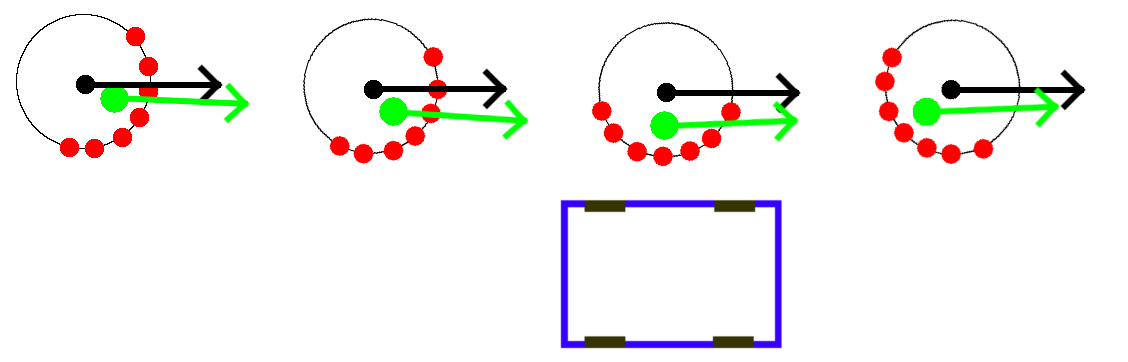
\includegraphics[height=40mm]{figures/raw/closing_ball.png}
	\caption{The closing ball}
	\label{closing_ball}
\end{figure} 

In figure \ref{closing_ball} this effect can be viewed. The ball is moving in a straight line, its speed vectors in every step are marked with the black arrows. The visible points (marked with red dots) are shifting to the side of the ball as it passes the car. As a result, the calculated speed vectors (green arrows) tend to 'bend' towards the car when the obstacles is getting closer.

The effect of the speed vectors changing does not seem relevant, but during motion planning, the ball is seen as an object that is moving forward, but suddenly, it starts to approach the car by turning more and more towards it, making all actuations get marked as unsafe.

The problems has not been solved entirely, but its effect has been reduced by changing the mass center calculation method in the mapping node.

